\documentclass[crop,tikz]{standalone}
\usetikzlibrary{backgrounds}
\colorlet{blue}{cyan}
\tikzset{
  inverted/.style = {
    color=white,
    background rectangle/.style={fill},
    show background rectangle
  }
}

\usepackage{amsmath,marvosym}
\tikzset{>=latex}
\usetikzlibrary{decorations.markings,positioning,arrows}
\colorlet{green}{green}

\begin{document}
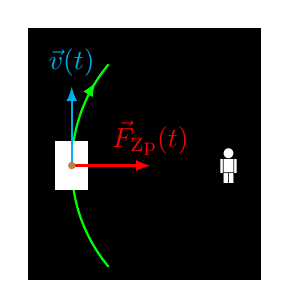
\begin{tikzpicture}[inverted,scale=2]
  \pgfmathsetmacro{\cx}{-1};
  \pgfmathsetmacro{\cy}{0};
  \pgfmathsetmacro{\cw}{0.2};
  \pgfmathsetmacro{\ch}{0.3};
  \pgfmathsetmacro{\angl}{40};
  \node at (0,0) {\LARGE\Gentsroom};
  \draw[thick,green,
        decoration={markings, mark=at position 0.9 with {\arrow{>}}},
        postaction={decorate}
  ] (180+\angl:1) arc (180+\angl:180-\angl:1);
  \coordinate (car) at (\cx,\cy);
  \draw[fill=white] (\cx-\cw/2,\cy-\ch/2) rectangle (\cx+\cw/2,\cy+\ch/2);
  \draw[->,blue,thick] (car) -- ++(0,0.5) node[above] {$\vec{v}(t)$};
  \draw[->,red,thick] (car) -- ++(0.5,0) node[above] {$\vec{F}_\text{Zp}(t)$};
  \draw[fill,brown] (car) circle (0.02);
\end{tikzpicture}
\end{document}
